\chapter{Literature Review}

This literature review examines the background and relevant technologies that form the foundation for the project, focusing on ROS2, its components, and the role of digital twins in robotic applications. 

\section{Digital Twin}
Digital Twin (DT) technology is an emerging field that continues to expand rapidly. Although many industries have begun adopting this technology, the definition of a Digital Twin remains ambiguous in the literature. Some authors define it as a virtual representation of a physical system, while others emphasize the exchange of information between two domains, incorporating sensors, data, and models \autocite{staczekDigitalTwinApproach2021}. In this report, the definition provided by the National Institute of Standards and Technology (NIST) will be used:

\begin{quote}
``A digital twin is the electronic representation—the digital representation—of a real-world entity, concept, or notion, either physical or perceived \autocite{voasDraftConsiderationsDigital2021}.''
\end{quote}

A DT functions as a model or simulation that offers static or dynamic views of its real-world counterpart. It integrates modeling, simulation, and real-time data to replicate the behaviour of its physical counterpart. Unlike static models, DTs are continuously updated in real-time.
The distinction between a DT and a mirroring system often overlaps, making it challenging to define a clear boundary. In this project, a digital twin is defined as a electronic representation of its real-world counterpart, capturing its electrical and functional characteristics. While both components can be controlled simultaneously, their behaviors remain distinct and unique to each system. Conversely, a mirroring system involves two counterparts that move synchronously, with the motion dictated either by the virtual model or the real-world robot.
DTs are applicable in various domains, such as simulating behaviour over time (Dynamic Modeling) or controlling physical systems through bidirectional communication, such as managing unmanned aerial vehicles (UAVs) or autonomous mobile robots (AMRs).
However, this technology introduces several challenges, including cybersecurity risks, heightened complexity, and ensuring the accuracy of the digital twin representation \autocite{voasDraftConsiderationsDigital2021}.


\section{Autonomous Robots}

An autonomous robot is defined as a system that can handle various environmental constraints automatically while completing a task. It is equipped with the necessary methods to adjust to its surroundings without requiring constant human input \autocite{wahdeINTRODUCTIONAUTONOMOUSROBOTS2016}. 
The predecessors of autonomous robots are conventional robots that are widely used in manufacturing across various industries for over two decades. Conventional robots operate by executing preprogrammed instructions or direct commands.
Autonomous robots are designed to increase flexibility and adaptability. These advanced systems can adapt to environmental constraints and perform tasks with minimal human intervention. 
A notable subclass of autonomous robots is mobile robots \autocite{fahimiAutonomousRobotsModeling2009}. 
In this project, the focus will lay on developing a digital twin of an autonomous mobile robot (AMR). AMRs, the latest advancement in unmanned mobile robots, are predominantly used in large warehouses for material handling. These robots are designed to move across a defined area and navigate through an environment to perform a specific task, while human intervention is kept at a minimum. Decisions on where and when to act are based on predefined programming and environmental inputs. 
In order to develop an AMR that is able to perform tasks autonomously a DT is essential. The open-source software ros2 offers a variety of a highly functional tool, which simplifies the process of building a DT significantly \autocite{staczekDigitalTwinApproach2021}.


%% CG: The entire ROS section should be placed in a separate chapter on the ROS2 architecture and concepts. After reading this part I would even consider it to be part of the method section.

\section{What is ROS?}

The robot operating system is an advanced open-source robotics software that provides a collection of software libraries and tools to help developers build robot software, offering features such as hardware abstraction, device drivers, libraries for commonly used algorithms, and message-passing between processes. 
The first version of ROS had a significant role in the maturing robot industry, the ROS ecosystem has become influential in nearly every intelligent machine sector.
The successor ROS2 was developed to address the limitations such as lack of security, low reliability in non-ideal environments and limited real-time support of its predecessor. The architecture of ROS2 is divided into three categories Middleware, Algorithms and Developer tools \autocite{macenskiRobotOperatingSystem2022}.

\subsection{What is a ROS distribution}

A distribution contains a collection of interrelated software components, tools, libraries and infrastructure that are bundled together and released at specific intervals. 
ROS as well as ROS2 are available in a sequence of distributions, these are essentially stable releases that include the core components which are required to build and run robotic systems. 
In the ROS ecosystem, there are two main types of distributions available: Long-Term Support (LTS) distributions and non-LTS (development) distributions. The main difference between the two lies in their update and maintenance policies.
LTS distributions are designed for stability and reliability, with updates provided at defined intervals, primarily focusing on bug fixes and security patches. The latest long-term support(LTS) distribution is the "Jazzy Jalisco", which was released on May 23rd, 2024 \autocite{openroboticsJazzyJaliscoJazzy}.

In contrast, non-LTS (development) distributions reflect the latest state of ROS development. This distribution includes the latest changes and features of ROS 2. Unlike other stable distributions, the non-LTS distribution is not focused on long-term stability but instead is constantly updated. It serves two purposes:

\begin{enumerate}
    \item It is a staging area for future stable distributions of ROS 2, and
%% CG: This is not a purpose
    \item It is a collection of the most recent development releases.
%% CG: This is a purpose ;)
    \item allows for testing existing solutions for upcoming ROS distributions.
\end{enumerate}

Due to it's frequent changes and potential instability it is not recommended for use in production environments. Within the ROS ecosystem, the rolling distribution takes on the role of the non-LTS (development) distributions \autocite{openroboticsDistributionsROS2a}.

\subsection{Nodes and Topics}

The simple explanation of a node is the following; nodes are executable files within a ROS2 package. Each node should be responsible for a single modular purpose. To send and receive data from other nodes, messages can be sent to a topic \autocite{openroboticsUnderstandingNodesROS}. A graphical overview of the interaction between nodes and topics is given in the figure~\ref{fig:Node_topics}. In order for this system to work properly the two nodes need to be accessible from the same network, further information regarding the network configuration will be discussed in the next chapter . 

\begin{figure}[h]
    \centering
    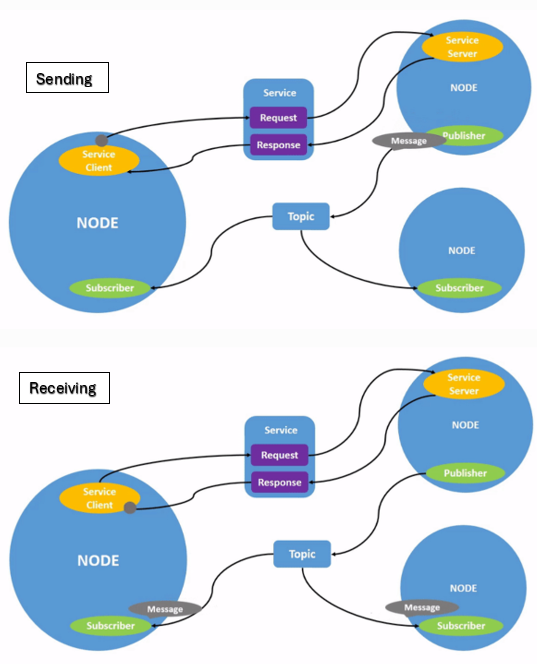
\includegraphics[width=0.7\textwidth]{Figures/Nodes_topics.png}
    \caption{URDF components relationships}
    \label{fig:Node_topics}
    \autocite{Interaction nodes and topics}
\end{figure}

\newpage
\section{Rviz and Gezebo}

ROS2 provides a variety of visualization and simulation tools, some developed within the ROS ecosystem and others designed to be compatible with it. Within the scope of this Project, the visualization tool RViz and the simulation tool Gazebo were chosen to support the development and implementation of the digital twin.

\subsection{RViz}
RViz is a ROS toolkit that enables the visualization of data and algorithms in real-world domains, including 2D and 3D spaces. It can work with various data structures, enabling its use across different computational and scientific fields. \autocite{kamRVizToolkitReal2015}

\subsection{Gazebo}

Gazebo is an open-source collection of modular software libraries aimed at simplifying the development of high-performance robotics and simulation applications.\autocite{openroboticsGazebo}

\subsection{Combination of RViz and Gazebo}

RViz itself does not provide a built-in simulation, therefore a parallel usage of Gazebo is widely used. Gazebo handles the physics-based simulation of robots and their environments, while RViz provides a real-time visual interface to display the simulation data. Together, they allow users to visualize the robot's movements, map generation, sensor data, and coordinate transformations, as well as to interact with the robot by sending commands or testing navigation and planning strategies in a controlled environment.\autocite{indriAMRSystemAutonomous}
In order to develop and implement a digital twin with the support of the two tools the robot's physical structure and configuration must be defined in a specific format.

\section{URDF, Xacro and SDF}

The Unified Robotic Description Format (URDF) is an XML file format used in ROS and ROS2 to define a robot's physical structure and configuration. It provides a 3D representation of the robot, specifying details about its joints, links, sensors, and their respective properties. This effectively describes the robot's physical design and behaviour. The diagram, as shown in Figure~\ref{fig:URDF_comp}, form the ROS wiki illustrates the relationships between these components \autocite{openroboticsUrdfROSWiki}.
URDF files are created to define the kinematic and dynamic properties of a single robot in isolation. 
To develop a more complex system, which includes sensors, actuators or a second robot most developers use the macro language xacro (XML macro). It enhances URDF files by allowing for conditional logic, variables, and parameterization, enabling developers to make these files configurable and maintainable. 
A Modular Xacro splits up the robot description into multiple separate child Xacro files, each with a specific purpose. These files are then included in a parent Xacro file. The modular structure typically includes:

\begin{enumerate}
    \item Robot Description File: Contains the main robot model description, such as links, joints, and kinematics.
    \item Material List File: Defines materials and visual properties, such as colors and textures used in the model.
    \item Configuration File: Includes parameters and settings required for simulation in tools like Gazebo, such as physical properties and plugin configurations.
\end{enumerate}

A Xacro file itself is an enhanced version of a URDF (Unified Robot Description Format) file, enriched with Xacro-specific tags to support macros, parameterization, and modular inclusion.
At runtime, the Xacro program preprocesses the parent Xacro file along with its included files to generate a standard URDF. This URDF file is then used by simulation tools (e.g., Gazebo) or visualization tools (e.g., RViz) \autocite{albergoUnderstandingXacroMisunderstandings2022}.
Another way to make URDF suitable for a gazebo simulation, without using Xacro, is to translate the URDF file to the native Simulation Description Format (SDF) of Gazbeo. The translation process includes the implementation of simulation-specific tags to the URDF file. These tags define attributes such as the robot's pose, friction, inertial elements, and other physical properties. Furthermore, these tags can describe the surroundings of the robot and thereby place the robot in a simulated world. 
Converting a URDF to SDF is straightforward and is achieved by adding Gazebo plugins to the URDF file. Essentially, Gazebo plugins create a communication interface (referred to as a Topic in ROS) between ROS and Gazebo. The control processes in ROS communicate through a Publish/Subscribe model on these Topics \autocite{takayaSimulationEnvironmentMobile2016}.

\begin{figure}[h]
    \centering
    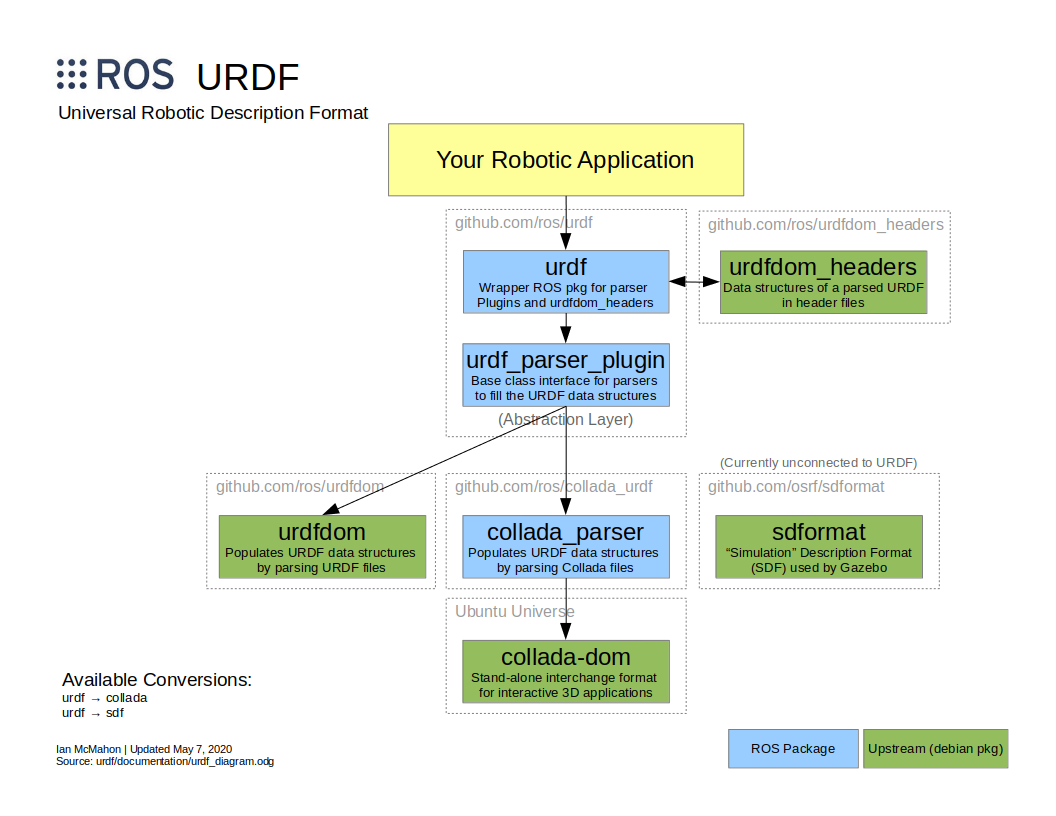
\includegraphics[width=0.7\textwidth]{Figures/urdf_diagram.png}
    \caption{URDF components relationships}
    \label{fig:URDF_comp}
\end{figure}
\autocite{openroboticsUrdfROSWiki}
